\section{Returning Results to the Frontend}
\label{sec:visitor}

As mentioned in \cref{sec:overview}, every command implementing the
\texttt{IReplCommand} interface returns an instance of a class implementing
the \texttt{IResult} interface. It is up to the frontend to determine how to
handle the result. Since commands can result in a failure or an exception (see
\cref{sec:function-comp}), it is not always clear what kind of
\texttt{IResult} the command returns.

To illustrate this, it is possible that a user tries to evaluate an input that
passes the parsing step but fails with an exception at the analyze step (see
\cref{fig:unit-flow}). The expected result is an \texttt{EvaluateResult},
but because an exception was thrown the corresponding wrapped
\texttt{AnalyzeUnit} cannot be created. The command that did the evaluation
then returns a \texttt{FailOrSuccessResult} containing the corresponding
\texttt{ExceptionResult} that caused the failure. However, the caller of the
command has no way of telling that the returned \texttt{IResult} is in fact a
\texttt{FailOrSuccessResult}.

\begin{figure}[t]
  \centering
  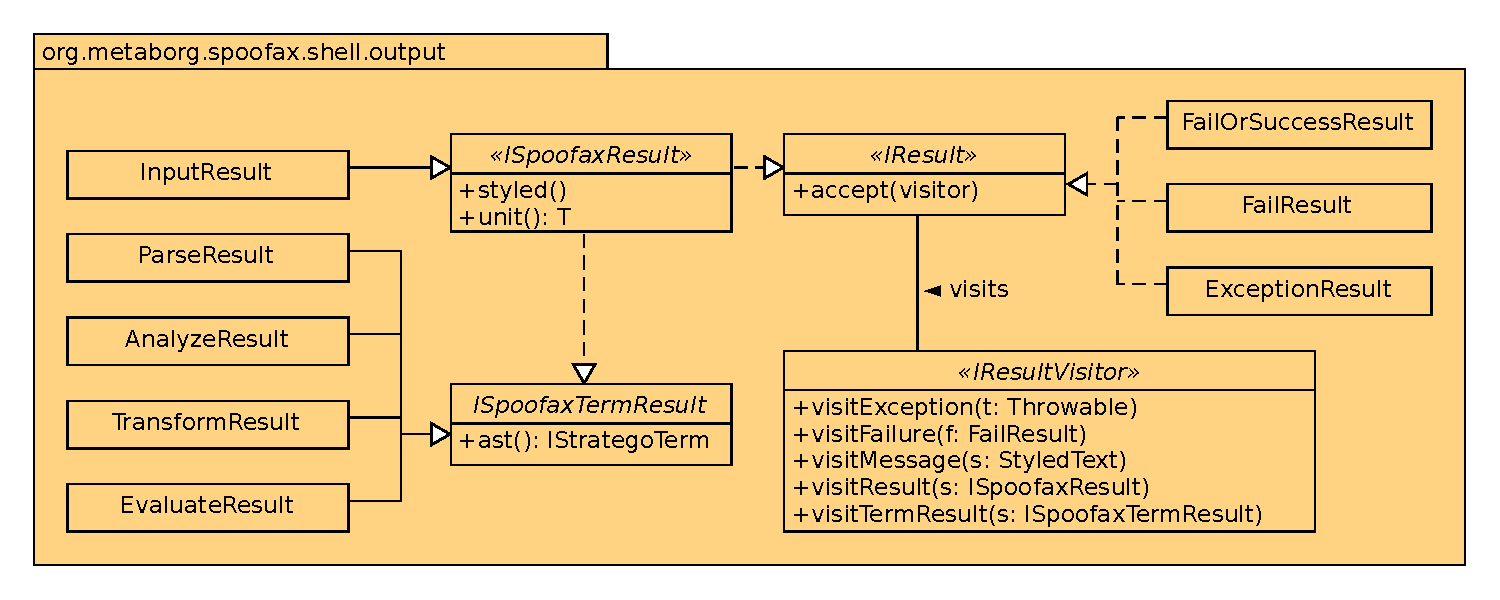
\includegraphics[width=0.8\textwidth]{uml-visitor}
  \caption{UML of the various concrete results and the result visitor.}
  \label{fig:uml-visitor}
\end{figure}

The visitor pattern has been adopted to solve this problem. As can be seen in
\cref{fig:uml-visitor}, every \texttt{IResult} can be ``visited'' by classes
implementing the \texttt{IResultVisitor} interface. Each subclass of
\texttt{IResult} decides what visitor method is called, and the
\texttt{IResultVisitor} gets a concrete subclass of \texttt{IResult} as argument
by means of double-dispatch. Furthermore, the \texttt{FailOrSuccessResult}
delegates the visitor to its wrapped \texttt{IResult}.

Implementations of the \texttt{IResultVisitor} can then decide per result type
how to handle the returned information. Since all commands can always return a
result with the original exception or the failed \texttt{ISpoofaxResult} by
returning a \texttt{FailOrSuccessResult}, the frontend is always provided with
error messages or the results of earlier processing steps.

The frontend has the responsibility to decide how to present the returned data
to the user, resulting in a lot of flexibility. However, this flexibility is not
always required. It is not necessary, for example, for a text-based console
REPL, although it can be used to easily highlight errors or print stack
traces. When integrating the REPL in multithreaded graphical user interface
(GUI) toolkits, however, this flexibility is very useful.

%%% Local Variables:
%%% mode: latex
%%% TeX-master: "../main"
%%% End:
